\documentclass[letterpaper, 10 pt, conference]{ieeeconf}

\usepackage{algorithm}
\usepackage[noend]{algpseudocode}
\usepackage{bm}

\usepackage{amsfonts}
\usepackage[pdftex]{graphicx}
\usepackage{comment}

\usepackage{caption}
\usepackage{subcaption}

%\usepackage{amsthm}
\newtheorem{thm}{Theorem}
\newtheorem{lem}{Lemma}
%\newtheorem{asmp}{Assumption}
\newtheorem{defn}{Definition}
%\newtheorem{clm}{Claim}

\IEEEoverridecommandlockouts                              % This command is only needed if 
                                                          % you want to use the \thanks command

\overrideIEEEmargins                                      % Needed to meet printer requirements.

\title{\LARGE \bf
Homotopy-Aware RRT$^{*}$ : Toward Human-Robot Topological Path-Planning
}

\author{
Daqing Yi, Michael A. Goodrich and Kevin D. Seppi
\thanks{Daqing Yi, Michael A. Goodrich and Kevin D. Seppi are with Department of Computer Science, Brigham Young University, Provo, UT, 84604, USA.
{\tt\small daqing.yi@byu.edu, mike@cs.byu.edu, kseppi@cs.byu.edu} }
}

\begin{document}


\maketitle
\thispagestyle{empty}
\pagestyle{empty}


%%%%%%%%%%%%%%%%%%%%%%%%%%%%%%%%%%%%%%%%%%%%%%%%%%%%%%%%%%%%%%%%%%%%%%%%%%%%%%%%
\begin{abstract}
Many researchers have noted that humans often represent the world using a topological rather than metric-based path-planning~\cite{kuipers99,aginsky1997two}, and various methods have been used to create topological-representations that can be used by path-planners for robots~\cite{mataric1992integration,thrun1998learning,fasola2013modeling,shah2013qualitative}.  
The idea of these planners is often to create algorithms that blend the benefits of graph-based path planners with the postulated topological representations used by a human partner or supervisor.
Such planners can produce paths consistent with well-reasoned topologies, but the planners may not work well in worlds that have sparse features or when the human intends a topological reference to be a ``soft'' constraint rather than a rigid path requirement. 
In this paper, we propose the HA-RRT$^{*}$, a homotopy-aware RRT$^{*}$, that explores the planning space for optimal solutions while respecting the path topology.
The paper restricts attention to problems where the goal is not only to optimize some objective but also contains ``soft'' or ``hard'' topological constraints, i.e. ``go quickly from A to B and better avoid C''.
Because the algorithm is aware of the homotopy class of each branch of the tree produced by the RRT$^{*}$ algorithm, the algorithm can enable a type of sliding autonomy for different levels of human's intent on the path topology.
Thus, a clear intent on the path topology provides the homotopic constraint, which reduces the working space of the optimal search; a vague intent on the path topology can be identified by comparing the optimal solutions in different homotopy classes.
The paper includes a set of simulation case studies and a corresponding theoretic analysis.
\end{abstract}

\begin{comment}
six pages
\end{comment}

%%%%%%%%%%%%%%%%%%%%%%%%%%%%%%%%%%%%%%%%%%%%%%%%%%%%%%%%%%%%%%%%%%%%%%%%%%%%%%%%
\section{Introduction}
\label{sec:intro}

An optimization problem is usually formed by a human who specifies a metric that attempts to encode task performance in a numerically amenable form.
As the task supervisor, the so-called {\em problem holder} in Woods' nomenclature~\cite{woods2004envisioning}, it is essential that the human's intent is correctly and precisely modeled.
%Optimality has been the most important heuristic in planning motions for the robots.
In planning a robot's motion for a task, the most common ways to model intent is with single numerical objective~\cite{6974170} or with multiple numerical objectives~\cite{yi2014supporting}.  Examples of objectives are many: Euclidean distance, minimum time, etc.
A numerical solver or calculus of variations is then used to generate a path that optimizes the given objectives.

Unfortunately, not all types of human intent can be easily modeled using common measurable objectives.
One difficult-to-model intent is the ``shape'' of the planned path.
Although shape properties like continuity and smoothness can be modeled using standard numerical constraints, shapes that refer to environment topology, such as ``go around building A and then between the two trees while avoiding region C,'' benefit from topological approaches.
In particular, concepts from algebraic topology can be used to create numerical representations of these topological desiderata or constraints.
In this paper, we present an algorithm that allows the human to specify avoiding regions, moving around objects, and satisfying constraints: via-point/waypoint constraints, reference path constraints~\cite{6974170} and temporal logic constraints~\cite{5650896}.

The topological concept of \emph{homotopy} is a mathematical formalism of the inherent similarity or dissimilarity of two paths.
Given two paths, if one can be deformed into the other without encroaching any obstacle, they are said to be \emph{homotopic}~\cite{Hernandez201544}.
The set of paths that are homotopic to each other form a \emph{homotopy class}, and the  set of homotopy classes partition the set of all possible paths between any two points $A$ and $B$.
In an environment containing obstacles, the homotopy partition can provide a useful way of grouping paths together based on the similarities of their ``shapes," where the term ``shape'' is interpreted using the formal topological notion.

Importantly, simple representative paths from within a homotopy class can often be associated with human intent.
Consider a path-planning problem where a human supervisor defines the task for a robot.
Further, consider the following list of ways in which a human can express intent about path shape, and the corresponding homotopy-based constraint:
%The task is needed to be modeled so that the robot can understand and plan for execution.
%Let the objective be only reaching to a target quickly, there can be several levels of how clear his intent is.
\begin{enumerate}
\item \emph{I want the path to visit a sequence of specific regions.}
Topologically, such a path is constrained to one homotopy class, so this homotopy class becomes the constraint of the optimization problem~\cite{Hershberger199463}.
%This homotopy class could be defined from a human initialized reference path.
\item \emph{I want the path to visit some regions and avoid other regions.}
Since it is possible that several homotopy classes can satisfy these requirements, the homotopic constraint restricts the path to  the set of homotopy classes that satisfy the requirements.
\end{enumerate}
The first two ways of expressing human intent translate into homotopic path constraints.
The next two allow a human to express preference among different path shapes, but also allow the human to tradeoff between following a desired path shape and optimizing another performance objective.
\begin{enumerate}
\setcounter{enumi}{2}
\item \emph{I prefer some path shapes over others, but I recognize that tradeoffs may be needed.} 
This indicates that the human has preferences over different homotopy classes, but also acknowledges that certain homotopy classes may not allow an acceptable optimization of another task-based objective.
If the preference on the homotopy classes can be modeled using an objective function, then non-dominant solutions over the task-based objective and homotopic objective can be found, and the human can select one of these solutions.
\item \emph{I have preferences over paths but I need help in understanding these preferences.}
In this case, the human's preference could be identified through an interactive process.
A straightforward way is for the planning algorithm to provide the best solution of each homotopy class to the supervisor.
The supervisor can then select one that satisfies his/her intent.
\end{enumerate}

In order to support these forms of human intent, expressed as homotopic constraints and preferences, we propose a homotopy-aware RRT$^{*}$ (HA-RRT$^{*}$) algorithm. 
This algorithm uses an RRT$^*$ algorithm to explore possible paths, but each branch of the random tree is aware of the homotopy class to which it belongs. 
The remainder of the paper presents this algorithm. We first review the relevant work in section~\ref{sec:related_work}.
We then introduce the algorithm in section~\ref{sec:algorithm} and show how it can be used to implement the different forms of human intent in section~\ref{sec:application}. 
An analysis of the algorithm is given in section~\ref{sec:analysis}, and then conclusions are presented.

\section{Related work}
\label{sec:related_work}

Humans often represent the world using a topological rather than metric-based path-planning~\cite{kuipers99,aginsky1997two}.
Various methods have been used to create topological-representations that can be used by path-planners for robots~\cite{mataric1992integration,thrun1998learning,fasola2013modeling,shah2013qualitative}.  
The obstacles in the map divides the paths into topological groups by the similarity.
The topological notion of homotopy presents a formal definition of the similarity between two paths.
This definition can be used both to determine the similarity between two paths as well as to partition paths into different classes.

Homotopy-based path planning requires an algorithm to determine the homotopic equivalence of two paths, which is usually computationally expensive.
There are a few research work that focus on effectively and efficiently identifying the homotopy class to which a path belongs or determining the homotopic equivalence of two paths.
%One straightforward way is constructing a set of reference frames in the map, so that the how a path crosses the frames can be used for identification. 
%A Voronoi diagram-based algorithm has been used to determine homotopy classes, but this algorithm shows limitations on finding some paths in some cases~\cite{banerjee2013framework}.
The Voronoi diagram is used to identify a path from any homotopy class in \cite{banerjee2013framework}.
By converting any path into a simple path from the Voronoi diagram, the homotopy class of the path can be determined.
However there exist limitations on finding some paths in complex obstacles in this approach.
%Specifically, generating Voronoi diagram for obstacles of complicated shapes is hard.
%By algebraic topology, the path of same homotopy class can be determined by using orientable band~\cite{Hershberger199463}.
By applying the funnel algorithm in the universal covering space, the minimum-length path is efficiently optimized in a given homotopy class in \cite{Hershberger199463}.
Similar with the Voronoi approach, the complexity of the problem is increased when the shapes of the obstacles are not smooth and convex.
Semi-algebraic cuts are used to convert the path into ``word'' so that the homotopic equivalence can be compared~\cite{Grigoriev:1998:PAS:281508.281528}.
The Cauchy Integral theorem has been introduced to determine the homotopic equivalence of any two paths by marking the positions in the obstacles as undefined~\cite{AAAI101920}.
Given two paths sharing the same start and goal, we can determine whether there is an obstacle inside a region that is closed by  two paths by the value of the complex integral.
Because the map is discretized, the computation cost expands greatly if the obstacles are reasonably approximated by the cells.

Sampling-based path planning, like the RRT or PRM algorithm, has been an effective and popular tool to plan paths.
The idea of homotopy has also been integrated when a sampling-based algorithm explores a given map by branching and reconfiguring its discrete structure of the world representation.
By homotopic redundancy, the paths from PRM could be categorized into different homotopy classes~\cite{1041613}.
By dividing the space using the rays crossing each obstacle, reference frames can be used to represent the paths as canonical sequences~\cite{Hernandez201544}.
In this way, the exploration process of the graph structure keeps tracking the homotopy class of the new branch in the tree structure so that the exploration process can be constrained in some homotopy classes.

The bidirectional RRT was originally proposed to accelerate the exploration process.
For a bidirectional RRT$^{*}$, the exploration process can still converge to the optimal solution with efficiency improvement
~\cite{Jordan.Perez.ea:CSAIL13}~\cite{starek2014bidirectional}.
With two trees exploring from two directions, 
the cost-to-go and the cost-to-arrive of a given position converge to the optimal.
It means that a solution, which is generated by connecting the subpaths from two trees with shared position, converges to the optimal solution that has the shared position as a via constraint.
It can be used to support the optimal search with the homotopic constraint.
We introduce the homotopy-aware bidirectional RRT$^{*}$ to support different level of intent on topology for the task supervisor.

\section{Homotopy-aware RRT$^{*}$}
\label{sec:algorithm}

%Without loss of generality, we only look at the minimization problem of the path planning.
Definition \ref{def:homo_path_planning} presents the homotopy-based optimal path-planning problem formed as a minimization problem.
%It can be extended into other homotopy-relevant optimal path planning.
\begin{defn}{ \textbf{Homotopy-Based Optimal Path-Planning} }
\label{def:homo_path_planning}
Consider a bounded, connected open set $ X \subset \mathbb{R}^{d} $, an obstacle space $ X_{\it obs} $, an initial state $ x_{init} $, and a goal state $ x_{goal} $. 
Denote the obstacle-free space by $ X_{\it free} = X \setminus X_{\it obs} $.
Define a {\em path} in $X$ as a continuous curve parameterized by $s$, denoted by $\sigma : [0,s] \rightarrow X$. 
Define the cost of the path as $ \mbox{\sc Cost} (\sigma) $.  
Define a set homotopy classes $ H \subseteq \bm{H} ( x_{init}, x_{goal} ) $, in which $ \bm{H} ( x_{init}, x_{goal} ) $ is the set of all the homotopy classes defined by $ x_{init} $ and $ x_{goal} $
\footnote{Theoretically there exists infinitely homotopy classes, because different ways of going around the obstacles.
In practice, only finite number of the homotopy classes should be considered.
In this paper, we only look at all the simple homotopy classes, which means we do not consider the homotopy class that goes around any obstacles in the optimization.}
.
The goal is to find paths $ \sigma^{*} \in \Sigma^{*}$ such that
\textit{ (a) } $ \forall \tau\in[0,s], \sigma^*(\tau) \in X_{\it free}$;
\textit{ (b) } $ \sigma^{*} (0) = x_{init} $ and $ \sigma^{*} (s) = x_{goal}  $; and
\textit{ (c) } $ \forall h \in H, \sigma^{*} = \min_{\sigma \in X_{\it free} \land h(\sigma^{*}) = h } \mbox{\sc Cost}  (\sigma) $. %; and
%\textit{ (d) } $ \sigma^{*}$ satisfies one or more homotopic constraints, defined below.
\end{defn} 

\begin{figure}[htbp]
	\centering
	\begin{subfigure}[t]{0.45\linewidth}
		\centering
		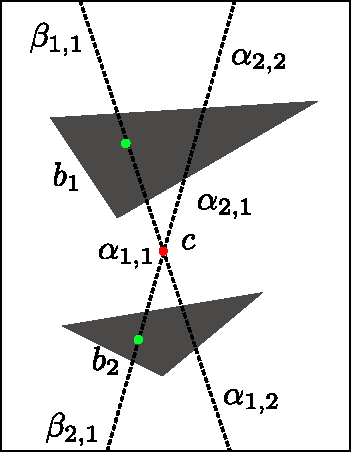
\includegraphics[width=\textwidth]{fig/obs_map.pdf}
		\caption{Decomposition of the map with obstacles.}
		\label{fig:obs_map:map}
	\end{subfigure}  
	%\\
	\begin{subfigure}[t]{0.5\linewidth}
		\centering
		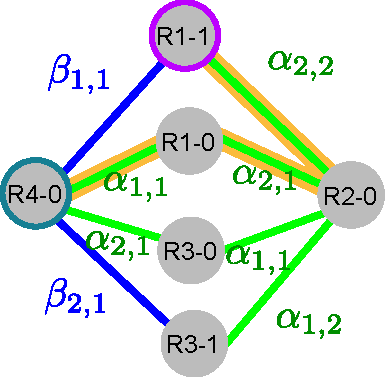
\includegraphics[width=\textwidth]{fig/obs_topology.pdf}
		\caption{The generated topological graph.}
		\label{fig:obs_map:topology}
	\end{subfigure}   
	\caption{Map with obstacles.}
	\label{fig:obs_map}
\end{figure}

To solve of the homotopy-based path planning, we need to figure out an efficient way to identify the homotopy class to which a path belongs.
In this paper, we use a set of reference frames for homotopy class identification.
Figure \ref{fig:obs_map:map} shows an example of a map that is decomposed with the reference frames(blue and green dash lines).
A \emph{reference frame} is defined as a line segment that connects either two obstacles or an obstacle and a boundary.
Thus crossing a reference reveals a position in between two corresponding obstacles or between an obstacle and a boundary.
Given the start position and the end position, how a path sequentially crosses the reference frames indicates the topology information.
Figure \ref{fig:obs_map:map} illustrates how the reference frames can be used to determine how a path (orange line) sequentially visits different regions.
Because the reference frames decompose the map into regions without overlaps, they can be generated from the Voronoi diagram.
However, in this paper, we adopt the improved Jenkins' method in \cite{Hernandez201544}.
The improved Jenkins' method provides a much simpler initialization process in complex obstacles than using Voronoi diagram, especially in the regions adjacent to the map boundary.
%It also avoids that the reference frames intersect with each other.
%As the reference frames are from the rays that rotate along the center point, the rotation order implies the direction of the path.

The reference frames decompose the map into several regions, which are the line segments formed by connecting the \emph{center point} $ c $ to a random \emph{obstacle point} $ b_{k} $ in each obstacle.
%{\sc This is ambiguous. Elaborate and use figure 1(a) to help describe how you form the line segments.} 
The obstacle point $ b_{k} $ is randomly sampled from the region of the obstacle $ B_{k} $.
The center point $ c $ is randomly sampled in $ X_{\it free} $, which is not in a line that connects any two different $ b_{k} $.

%Observe how this process partitions the space $X$ into distinct regions, but note that the partition of $X$ differs from the partition of all possible paths through the space created by grouping paths into homotopic classes. 
%We use the partition of $X$ to identify a homotopic class as follows, again using the improved Jenkins' method.

Let $ \bm{B} $ denote the set of obstacles and $ B_{k} $ denote one of the obstacles.  
The generation of the reference frame is given in Algorithm \ref{alg:harrt:init_ref_frames}, which returns a set of reference frames $ \bm{R} $.
The called methods in Algorithm \ref{alg:harrt:init_ref_frames} are explained as following,
\begin{itemize}
	\item \textsc{Line}($ p_{1}, p_{2} $):
	Return a line that is defined by $ p_{1} $ and $ p_{2} $.
	\item \textsc{Ray}($ p, \vec{d} $):
	Return a ray that starts from $ p $ with direction $ \vec{d} $.
	\item \textsc{Intersect}($ r , \bm{B} $):
	Return line segments by cutting a line $ r $ using the obstacles $ B $.
\end{itemize}
%{\sc What is B?}


\begin{algorithm}[hbtp]
	\begin{algorithmic}[1]
		\State $ \bm{R} = \emptyset, \bm{b} = \emptyset, \bm{\alpha} = \emptyset, \bm{\beta} = \emptyset $
		\For{\textbf{each} $ B_{k} \in \bm{B} $ }
		\State $ b_{k} $ $ \leftarrow $ Randomly sample from $ B_{k} $
		\State $ \bm{b} \leftarrow \bm{b} \cup b_{k} $
		\EndFor
		\While{ $ \exists b_{k}, b_{k'} , c \in $ \Call{Line}{ $ b_{k}, b_{k'} $ } }
		\State $ c \leftarrow  $ Randomly sample from $ \bm{X}_{free} $
		\EndWhile
		\For{\textbf{each} $ b_{k} \in \bm{b} $ }
		\State $ \alpha_{k} \leftarrow $ \Call{Ray}{ $ b_{k}, c - b_{k} $ }
		\State $ \beta_{k} \leftarrow $ \Call{Ray}{ $ b_{k}, b_{k} - c $ }
		\State $ \bm{\alpha} \leftarrow \bm{\alpha} \cup \alpha_{k} $
		\State $ \bm{\beta} \leftarrow \bm{\beta} \cup \beta_{k} $			
		\EndFor
		\For{\textbf{each} $ \alpha_{k} \in \bm{\alpha} $}
		\State $ \{ \alpha_{k_{m}} \} \leftarrow $ \Call{Intersect}{$ \alpha_{k}, \bm{B} $}
		\State $ \bm{R} \leftarrow \bm{R} \cup \{ \alpha_{k_{m}} \} $
		\EndFor
		\For{\textbf{each} $ \beta_{k} \in \bm{\beta} $}
		\State $ \{ \beta_{k_{m}} \} \leftarrow $ \Call{Intersect}{$ \beta_{k}, \bm{B} $}
		\State $ \bm{R} \leftarrow \bm{R} \cup \{ \beta_{k_{m}} \} $
		\EndFor
		\Return $ \bm{R} $
	\end{algorithmic}
	\caption{ \textsc{InitRefFrames} ($ \bm{X}_{free} , \bm{B} $) }
	\label{alg:harrt:init_ref_frames}
\end{algorithm} 

Figure \ref{fig:obs_map:map} illustrates an example of the generated reference frames of a map.
$ b_{1} $ and $ b_{2} $ are randomly sampled from each obstacles.
Then a center point $ c $ is randomly sampled, which does not locate in any line connects any two $ b_{k} $.
For each $ b_{k} $, two rays are generated from two directions, $ \alpha_{k} $ is towards the center point $ c $, $ \beta_{k} $ is the reserved direction.
Both $ \alpha_{k} $ and $ \beta_{k} $ intersect with the obstacles $ B $, the generated line segments of which are the reference frames.
More details can be found in \cite{Hernandez201544}.

A topological graph can be created by the connectivity of the decomposed regions.
Each region from the map decomposition is a node in the topological graph.
Each reference frame is adjacent to two regions, thus it becomes an edge that connects two nodes.
Figure \ref{fig:obs_map:topology} shows a topological graph from the map decomposition in Figure \ref{fig:obs_map:map}.
%By the connectivity of the regions, we can generate a topological graph.
%{\sc Explain how.  Essentially, each region in the partition of $X$ created by Jenkins' method is a vertex in the graph.  Edges between vertices are added between vertices if the vertices represent adjacent regions.}
%The nodes are the regions and the edges are the reference frames. 
%{\sc What do you mean "reference frame"?  This term hasn't been defined.}

Given two paths, how they sequentially cross the reference frames indicate the homotopy equivalence.
Any path that sequentially visits the regions can be mapped to a node walk on the topological graph.
It is noticeable that two adjacent regions might be connected with not only one reference frame, which means that two nodes in the topological graph might be connected with more than one edge.
Thus, two paths with same edge sequence belong to same homotopy class but two path with same node sequence don't.
We select the sequence of the visited reference frames instead of the sequence of the visited regions to represent the homotopic information.
%Any path can be mapped into a sequence of nodes in the topological graph.  
%{\sc Explain how or given an example.}
%In determining the homotopy class, two paths share same start and goal.
%Thus they can be compared also by using only the visited edges, which are equivalent with the crossed reference frames. 
%{\sc Again, "reference frame" hasn't been adequately defined.  I believe it is the boundary between two regions.}
%Assign each reference frame a {\em character}. 
%{\sc Equivalently, assign each edge a character.}
%It is noticeable that the 
Label each reference frame with a \emph{character}.
Each path can be mapped into a {\em string}, which represents the sequence of the crossed reference frames.
In \cite{Hernandez201544}, the string is used to identify the homotopy class of each branch in the RRT so that the growth of a tree is constrained in a homotopy class.
Because starting from the root of the tree to each branch makes a subpath.
In this paper, each branch of the tree structure tracks the corresponding string as the homotopy information so that the homotopic constraints can be satisfied or the homotopy class can be identified.
We define the paths with same string as a \emph{string class}.
Two string classes might still belong to same homotopy class, e.g. a string class $ \alpha_{1,1}-\alpha_{2,1} $ and a string class $ \alpha_{2,1}-\alpha_{1,1} $ by the reference frames in Figure \ref{fig:obs_map}.
A homotopic grammar is needed to identify the equivalence.
Also the homotopic grammar can be used to find all the equivalent string classes in the same homotopy class by giving one string class.
The definition of the homotopic grammar will be discussed in Section \ref{sec:homotopic_grammar}.

%The string is used for the homotopy awareness in this paper, which inherits from \cite{Hernandez201544}.

%{\sc Do you explain how the string indicates the homotopy class?  
%The term ``homotopy awareness" is not defined adequately, and I suggest avoiding it.  

%Stating that some property of the algorithm ``inherits from [some reference]" doesn't explain to the reader %what you did. Are you just saying that we are describing how to algorithm in the reference works?  If so, say that instead of "inherits from."}


%{\sc So, is $\mathbf{R}$ the set of unique characters assigned to the edges of your graph? Is $\mathbf{B}$ the set of regions in the world, so each $B_k \in \mathbf{B}$ is a region?}
%{\sc How is $c$ sampled in line 6? What is $\mathbf{b}$ and how is it initialized -- line 4.}

With the generated reference frames $ \mathbf{R} $ to identify the homotopy classes, the next question is how to search the optimal paths in the homotopy classes.
The RRT$^{*}$ explores the map to generate an optimal tree structure based on the cost distribution in the map.
The homotopy-based path planning problem essentially searches for the optimal solutions with the constraints of visiting different regions, which a single optimal tree structure only explore the only best and cannot support.
Here, we use a bidirectional RRT$^{*}$ to obtain the optimal cost-to-come and cost-to-go for different positions.
We can eventually have the optimal path from the start to the goal via some position by combining the optimal cost-to-come to this position and the optimal cost-to-go to this position.
Because the string classes of the branches of both two trees are also tracked in the exploration process, the optimal path that visits a specific position can be used to update the optimal paths of the string classes. 
Because the string class is tracked during the exploration process, the homotopy class to which a branch of the tree belongs is aware.
The proposed algorithm is named Homotopy-aware RRT$^{*}$ (HA-RRT$^{*}$).
The exploration process is given in Algorithm \ref{alg:harrt}.

Two trees, the \emph{start tree} $ G_{s} $ and the \emph{goal tree} $ G_{g} $, are constructed from $ x_{init} $ and $ x_{goal} $ respectively.
Two trees explore the map bidirectionally by calling \textsc{Explore}(), defined in Algorithm \ref{alg:harrt:explore}, at each iteration.
By using each new vertex returned from \textsc{Explore}(), we can call \textsc{Connect}() to create a path with a vertex in the other tree.
The created path will be compared with the current best path that belongs to the same string class.
If it is a better one, the best path in this string class will be updated, which is implemented in \textsc{UpdateBestPathByClass}().

\begin{algorithm}[hbtp]
	\begin{algorithmic}[1]
		\State $ i \leftarrow 0 $
		\State $ V_{s} \leftarrow \{ x_{init} \} $; $ E_{s} \leftarrow \emptyset $; $ G_{s} \leftarrow (V_{s}, E_{s}) $
		\State $ V_{g} \leftarrow \{ x_{goal} \} $; $ E_{g} \leftarrow \emptyset $; $ G_{g} \leftarrow (V_{g}, E_{g}) $
		\While{ $ i < N $ }
			\State $ G_{s}, x_{s}^{new} \leftarrow $ \Call{Explore}{$ G_{s}, i $}
			\State $ G_{g}, x_{g}^{new} \leftarrow $ \Call{Explore}{$ G_{g}, i $}
			\State $ p_{s} \leftarrow $ \Call{Connect}{$  x_{s}^{new}, G_{g} $}
			\State $ p_{g} \leftarrow $ \Call{Connect}{$  x_{g}^{new}, G_{s} $}
			\State $ P \leftarrow $ \Call{UpdateBestPathByClass}{$ p_{s}, P $}
			\State $ P \leftarrow $ \Call{UpdateBestPathByClass}{$ p_{g}, P $}
			\State $ i \leftarrow i + 1 $
		\EndWhile
		\State $ P \leftarrow $ \Call{MergePaths}{$ P $}
		\Return $ P $
	\end{algorithmic}
	\caption{HA-RRT$^{*}$ ($ x_{init} , x_{goal} $) }
	\label{alg:harrt}
\end{algorithm}


\begin{algorithm}[hbtp]
	\begin{algorithmic}[1]
		\State $ x_{rand} \leftarrow $ \Call{ Sample }{$ i $} ;
		\State $ x_{nearest} \leftarrow $ \Call{Nearest}{$ G, x_{rand} $}
		\State $ x_{new} \leftarrow $ \Call{Steer}{$ x_{nearest}, x_{rand},\eta $}
		\If{ \Call{ObstacleFree}{$ x_{nearest}, x_{new} $} }
			%\State $ G \leftarrow $ \Call{ Extend }{$ G, x_{new}, x_{\it nearest} $}
			\State $ x_{min} \leftarrow x_{nearest} $
			\State $ X_{near} \leftarrow $ \Call{Near}{$ G, x_{new}, | V | $}
			\State $ s \leftarrow $ \Call{STR}{$x_{new}$} $ \cup $ \Call{CRF}{$ ( x_{new}, x_{near} ), \bm{B} $}
			\If{\Call{HomotopyCheck}{$ s $}}
				\For{\textbf{each} $ x_{near} \in X_{near} $ }
					\If{ \Call{ObstacleFree}{$ x_{new} , x_{near} $} }
						\If{ \Call{Cost}{$ x_{near} $} $ + c( $ \Call{Line}{$ x_{near}, x_{new} $} $ ) < $ \Call{Cost}{$ x_{new} $} } 
							\State $ x_{min} \leftarrow x_{near} $
						\EndIf
					\EndIf
				\EndFor

				\State $ E' \leftarrow E' \cup \{ ( x_{min}, x_{new} ) \} $
				\For{\textbf{each} $ x_{near} \in X_{near} \setminus \{ x_{min} \} $ }
					\If{\Call{ObstacleFree}{$ x_{new} , x_{near} $} and \Call{Cost}{$ x_{near} $} $ > $ \Call{Cost}{$ x_{new} $} + c(\Call{Line}{$ x_{new}, x_{near} $}) }
					   \State $ s \leftarrow $ \Call{STR}{$x_{new}$} $ \cup $ \Call{CRF}{$ ( x_{new}, x_{near} ), \bm{B} $}
					   \If{\Call{HomotopyCheck}{$ s $}}
					   		\State $ x_{parent} \leftarrow $ \Call{Parent}{$ x_{near} $}
							\State $ E' \leftarrow E' \setminus \{ ( x_{parent}, x_{near} ) \} $
							\State $ E' \leftarrow E' \cup \{ ( x_{new}, x_{near} ) \} $
					   \EndIf
					\EndIf
				\EndFor	
			\EndIf
		\EndIf
		\Return $ G, x_{new} $
	\end{algorithmic}
	\caption{ \textsc{Explore}($ G, i $) }
	\label{alg:harrt:explore}
\end{algorithm}

The exploration process of a tree structure is similar with that in the RRT$^{*}$~\cite{Karaman-RSS-10}, 
which is organized and described in the \textsc{Explore}() procedure in this paper.
The only difference is that the string of each branch is updated and there is the \textsc{HomotopyCheck}() to check whether the string of a branch is a substring of one reference strings.
The called methods in Algorithm \ref{alg:harrt:explore} are defined as following:
\begin{itemize}
	\item \textsc{CRF}($ l, \bm{R} $):
	Returns the character that represents the crossed reference frames if any.
	\item \textsc{STR}($ x $):	
	Returns the string that represents the crossed reference frames sequentially.
	%\item \textsc{HomotopyCheck}{($ s $)}
	%Returns if the path or subpath $ s $ satisfies a given homotopy constraint.
\end{itemize}

Because the RRT$^{*}$ maintains a tree structure, each vertex has only one path to arrive from the root.
This path, which starts from the root to the vertex, indicates a string of characters sequentially.
Each character represents a crossed reference frame.
If the string of a branch is not a substring of a reference string, extending the branch cannot make a path that generates the reference string.
The \textsc{HomotopyCheck}() guarantees that a new node is added or rewired only when the string of the new branch is a substring of one reference string.
For example, if the reference string is defined as $ A-B $, a branch with string $ A $ satisfies the constraint but a branch with string $ B $ doesn't.
The reference strings are generated by the equivalence of a given homotopy class defined by the homotopic grammar.
Indirectly, the homotopic constraint can be guaranteed by using the \textsc{HomotopyCheck}().
%{\sc How?}
%The homotopy constraint is defined as a \emph{homotopic grammar}.
%{\sc New concept.  You need to introduce a concept and explain something about it before you use it, or you must tell the reader what purpose the concept serves {\bf and} that you will explain it later in the paper.} 
%{\sc Need to explain  this better.}

The \textsc{Connect} procedure connects a vertex with the other tree to generate a path from the start to goal.
In order to guarantee optimality, a set of near vertices is provided to find the best vertex to be connected with.
The methods in Algorithm \ref{alg:harrt:binding} are defined as following:
\begin{itemize}
	\item \textsc{Path}($ v, G $):	
	Returns the path from the root of $ G $ to the vertex $ v $.
	\item \textsc{Concatenate}{($ p_{a}, p_{b} $)}
	Returns a concatenated path of $ p_{a} $ and $ p_{b} $.
	If $ p_{a} $ and $  p_{b} $ are from different directions, one of the them will be reversed for the concatenation.
\end{itemize}

\begin{algorithm}[hbtp]
	\begin{algorithmic}[1]
		\State $ p_{min} = \emptyset $
		\State $ X_{near} \leftarrow $ \Call{NEAR}{$ G, x_{new}, |V| $}
		\For{\textbf{each} $ x_{near} \in X_{near} $ }
		    \If{ \Call{ObstacleFree}{$ x_{new}, x_{near} $} } 
			    \If{ $ x_{new} \in G_{s} $ }
					\State $ p \leftarrow $ \Call{Concatenate}{$  x_{new} ,  x_{near} $}
				\Else
				    \State $ p \leftarrow $ \Call{Concatenate}{$  x_{near}, x_{new} $}			
				\EndIf
			    \If{ \Call{HomotopyCheck}{$ p $} and $ c( p ) < c( p_{min} ) $ }
			    	\State $ p_{min} = p $
			    \EndIf 
			\EndIf
		\EndFor
		\Return $ p_{min} $
	\end{algorithmic}
	\caption{ \textsc{Connect}($ x_{new}, G $) }
	\label{alg:harrt:binding}
\end{algorithm}

Because both the start tree $ G_{s} $ and the goal tree $ G_{g} $ add a new vertex. 
The \textsc{Connect}() procedure creates a path by connecting the new vertex with the other tree, which are $ p_{s} $ and $ p_{g} $ correspondingly.
The new paths will be used to update the best path of the string classes to which they belong in \textsc{UpdateBestPathByClass}().

When the exploration process is finished, there is a set that contains the best paths for all the string classes.
Because we are interested with the optimal paths in all the homotopy classes.
We need to merge the optimal paths in the string classes that belongs to same homotopy class.
The \textsc{MergePaths}() procedure will be called to merge the equivalent string classes into the same homotopy classes. 
Thus the set of paths $ P $ will be updated.
We can have the optimal paths of all the homotopy classes under given homotopic constraint.

\section{Analysis}
\label{sec:analysis}

The HA-RRT$^{*}$ consists of the homotopy-aware exploration and the constrained optimization.
In this section, we look at how to have better support on the homotopy classes and provide the constrained optimal guarantee.

\subsection{homotopic grammar}
\label{sec:homotopic_grammar}

The reference frames do not have any intersection between each other so that the map can be divided into regions without overlap.
Any path in the map belongs to a string class by how it sequentially crosses the reference frames.
In a homotopy-based path planning problem, given the start position and the goal position, we have a structural rule of how the string should be like, which is defined as the homotopic grammar.


\begin{figure}
	\centering
	\begin{subfigure}[t]{0.4\linewidth}
		\centering
		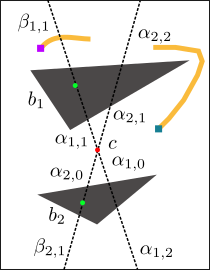
\includegraphics[width=\textwidth]{fig/feasibility}
		\caption{Feasibility}
		\label{fig:grammar:feasibility}
	\end{subfigure}  
	\begin{subfigure}[t]{0.4\linewidth}
		\centering
		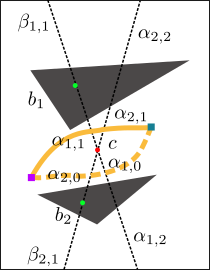
\includegraphics[width=\textwidth]{fig/equivalence}
		\caption{Equivalence}
		\label{fig:grammar:equivalence}
	\end{subfigure}
	\\
	\begin{subfigure}[t]{0.4\linewidth}
		\centering
		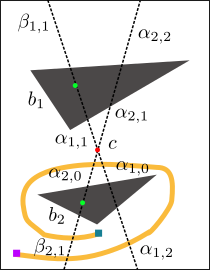
\includegraphics[width=\textwidth]{fig/recurring}
		\caption{Recurring}
		\label{fig:grammar:recurring}
	\end{subfigure}  
	\begin{subfigure}[t]{0.4\linewidth}
		\centering
		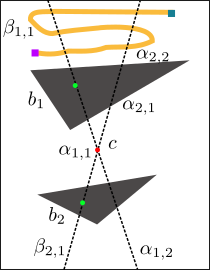
\includegraphics[width=\textwidth]{fig/repeated_pattern}
		\caption{Palindrome pattern}
		\label{fig:grammar:palindrome_pattern}
	\end{subfigure} 
	\caption{Homotopic grammar.}
	\label{fig:grammar}
\end{figure}

The homotopic grammar defines the acceptable strings, the equivalence of the strings in homotopy and other relevant shape information.
The grammar can be represented by a finite state machine, which is constructed from the topological graph.
The region that the start position is in defines the initial state.
The region that the goal position is in defines the end state.
\begin{itemize}
	\item \textbf{Feasibility}
	As the reference frames are connected by the regions, any strings generated from the grammar must be a feasible one in the map.
	A feasible string means that any two sequential characters of it are connected in the topological graph by the nodes of the regions.
	An example is given in Figure \ref{fig:grammar:feasibility}.
	A string of $ \beta_{1,1} $ cannot be from a correct path from the region that the start position is in to the region that the goal position is in.
	The finite state machine can be used to check whether a string is accepted by the homotopic grammar, which indicates that the string of a path is a feasible one.
	
	\item \textbf{Equivalence}
	Some characters of the reference frames are equivalent in constructing the strings.
	This property usually lies in the reference frames that are intersected with each other.
	In the Jenkins' method, all the reference frames contain the center point $ c $ show this property.
	The segment crossing those reference frames in any sequence belongs to same homotopy class.
	Figure \ref{fig:grammar:equivalence} shows an example.
	A path in string class $ \alpha_{1,1}-\alpha_{2,1} $ and a path in string class $ \alpha_{2,0}-\alpha_{1,0} $ belong to the same homotopy class.
	
	\item \textbf{Recurring character}
	Recurring character in a string indicates that the path goes around some obstacles and back to cross a visited region, if the substring between the recurring characters is not palindrome.
	One example is illustrated in Figure \ref{fig:grammar:recurring}.
	A string $ \beta_{2,1}-\alpha_{1,2}-\alpha_{1,0}-\alpha_{2,0}-\beta_{2,1} $ contains the recurring of $ \beta_{2,1} $, which indicates that a path crosses a reference twice.
	It usually means that the path goes back to a visited region again.
	These types of path topologies might be required in some complicate tasks.
	
	\item \textbf{Palindrome pattern}
	Palindrome pattern is a particular case of recurring character.
	It shows that the path is back and forth among some regions,
	which is very important in checking the equivalence of two string classes.
	In minimization problem, it is not useful and can be often ignored.
	Because a palindrome pattern will only increase the cost if the cost function is additive.
	However, in some special scenario, for example it is expected to scan a region for a fixed number of times, the palindrome pattern can be used.
	
	In Figure \ref{fig:grammar:palindrome_pattern}, the string $ \beta_{1,1}-\alpha_{2,2}-\alpha_{2,2}-\beta_{1,1}-\beta_{1,1}-\alpha_{2,2} $ contains a palindrome structure $ \beta_{1,1}-\alpha_{2,2}-\alpha_{2,2}-\beta_{1,1} $.
	It can be removed in determining the homotopy equivalence.
	Thus it equals to the string $ \beta_{1,1}-\alpha_{2,2} $.
	
\end{itemize}

\subsection{Optimality with constraint}
\label{sec:optimality_constraint}

The way that the RRT$^{*}$ algorithm works is that it incrementally constructs a tree from the root position.  
The cost of the path from the position of the root node to the positions of every other node converges to the minimal possible cost between the positions as the number of iterations approaches infinity.  
We restate this as a lemma, and note that the corresponds exactly to that given for Theorem 22 in~\cite{Karaman-RSS-10}.
\begin{lem}
	\label{lem:tree_vex:conv}
	Given Assumptions 1-3 in \cite{Karaman-RSS-10},
	the cost of the minimum cost path from the root to any vertex in the RRT$^{*}$ converges to the optimal cost almost surely.
\end{lem}

The HA-RRT$^{*}$ uses bidirectional trees to explore the map.
In the \textsc{Connect}() procedure, a vertex $ v $ in either $ G_{s} $ or $ G_{g} $ is used to create a path by connecting with another vertex in the other tree.
If we see the position of $ v $ as a via-point of the paths, we can have the asymptotic optimality with the set of paths has $ v $ as via-point.
It is stated in Lemma \ref{lem:optimal_via_point}.

\begin{lem}
	\label{lem:optimal_via_point}
	Given Assumptions 1-3 in \cite{Karaman-RSS-10},
	the path concatenated from a path from $ G_{s} $ for $ v $ and a path from $ G_{g} $ for $ v $ converges to the optimal path through $ v $ almost surely. 
	
	\begin{proof}
		Look at connecting a vertex $ v_{s} $ in $ G_{s} $ with the $ G_{g} $.
		Let $ c (v_{s}) $ denote the cost of the $  v_{s}  $ in $ G_{s} $, which is the cost-to-come from the start to the position of $  v_{s} $.
		Let $ v_{g} $ be the vertex to be connected in $ G_{g} $.
		Let $ c ( v_{g} ) $ denote the cost of the $  v_{g} $ in $ G_{g} $, which is the cost-to-come from the goal to the position of $  v_{g} $.
		It equals to the cost-to-go from the position of $ v_{g} $ to the goal.
		Let $ \sigma_{G_{s},G_{g}} (v_{s}, v_{g}) $ be a path concatenated by two sub-paths from $  v_{s} $ and $  v_{g} $. 
		Its cost $ \mbox{\sc Cost} (\sigma_{G_{s},G_{g}} ( v_{s}, v_{g} )) =  c (v_{s}) + c (v_{g}) + c (\mbox{\sc Line} (v_{s}, v_{g}) ) $.
		By Lemma \ref{lem:tree_vex:conv}, we know that $ c (v_{s}) $ and $ c (v_{g}) $ converge to optimal almost surely.
		$ c (\mbox{\sc Line} (v_{s}, v_{g})  ) $ will also converge, because $ v_{g} $ is selected from a set of near vertices.
		Thus, the cost of $ \sigma_{G_{s},G_{g}} (v_{s}, v_{g}) $ converges to optimal almost surely. 
		Similarly, we can have the same result on connecting a vertex $ v_{g} $ in $ G_{g} $ with the $ G_{s} $.
	\end{proof}
\end{lem}

By Lemma \ref{lem:optimal_via_point} we can have Theorem \ref{thm:constrained_optimality} and Theorem \ref{thm:homotopy_pref:optimal}.
Theorem \ref{thm:constrained_optimality} and Theorem \ref{thm:homotopy_pref:optimal} guarantee that the applications mentioned in Section \ref{sec:application} can find the optimal solutions as stated.

\begin{thm}
	\label{thm:constrained_optimality}
	Given Assumptions 1-3 in \cite{Karaman-RSS-10},
	the HA-RRT$^{*}$ can find the optimal path in one simple homotopy class almost surely.
\end{thm}

\begin{thm}
	\label{thm:homotopy_pref:optimal}
	Given Assumptions 1-3 in \cite{Karaman-RSS-10}, 
	the HA-RRT$^{*}$ can find all the non-dominated paths when the topology is an objective.
\end{thm}


\section{Homotopy-aware optimal path planning}
\label{sec:application}

By the homotopy-aware exploration process, the HA-RRT$^{*}$ can return optimal paths of different homotopy classes with given homotopy constraints.
In this section, we show the sliding autonomy in different levels of the human's intent on the topology by using the HA-RRT$^{*}$.

\subsection{Homotopic constraint from a reference path}
\label{sec:string_constraint}

In planning a path for a task, if the human has a determined mind of how the topology of the path should be, the HA-RRT$^{*}$ can help to find the optimal path in all the paths of a given topology.
By an interactive process, the human can initialize a reference path to represent the topology from his/her intent, which defines a homotopy class.
The homotopy-based optimal path planning becomes finding the optimal path in a given homotopy class.
The given homotopy class is the constraint.
Because the HA-RRT$^{*}$ only returns single solution that is the optimal path in this homotopy class, a single-directional tree structure is enough to explore the regions.

\begin{figure}
	\centering
	\begin{subfigure}[t]{0.47\linewidth}
		\centering
		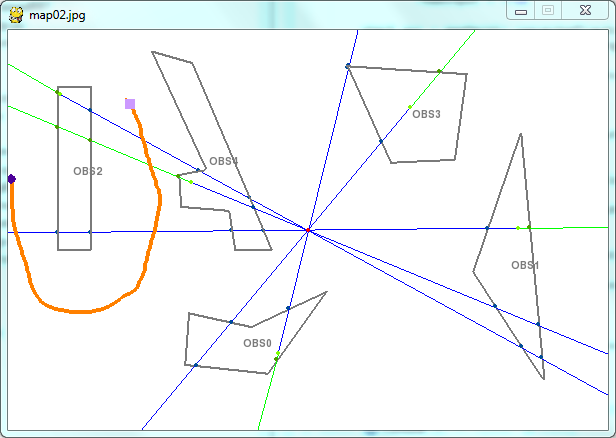
\includegraphics[width=\textwidth]{fig/referenceHomotopy.png}
		\caption{Reference path}
		\label{fig:reference_path:reference}
	\end{subfigure}  
	%\\
	\begin{subfigure}[t]{0.47\linewidth}
		\centering
		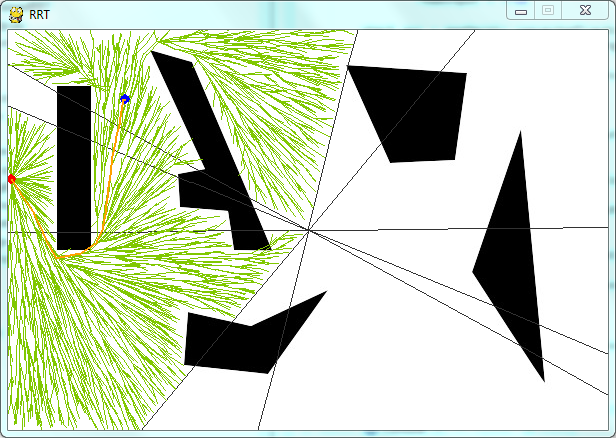
\includegraphics[width=\textwidth]{fig/homotopicConstrainedRRT.png}
		\caption{RRT$^{*}$ with homotopic constraint}
		\label{fig:reference_path:rrt}
	\end{subfigure}   
	\caption{Homotopic constraint from a reference path.}
	\label{fig:reference_path}
\end{figure}

In this case, it is sometimes fair to assume that the optimal path of a homotopy class is known as the optimal path of all the string classes in the homotopy class in the minimization problem.
It indicates that the optimal path only sequentially visits several regions by the string.
Then, the exploration of the tree can be only in the relevant regions.
Because of the reduced working space and the single-directional tree structure, the search efficiency should be increased.

Figure \ref{fig:reference_path} gives an example.
A user firstly initializes a reference path, which indicates the intended homotopy class as in Figure \ref{fig:reference_path:reference}.
Assume that the optimal path is known in the string class of the reference path.
The string of the reference path is then applied as the constraint.
A single-directional tree is then used to explore only the relevant regions under this constraint, as shown in Figure \ref{fig:reference_path:rrt}.
If more than one string classes in the same homotopy class are hoped to be checked, more relevant regions are then needed to be explored.


\subsection{Homotopic constraints from required/forbidden regions}
\label{sec:region_constraint}

In planning a path for a task, if the human only can tell several regions that should be avoided or several regions that are required to visit, the HA-RRT$^{*}$ explores the paths that satisfies the defined constraints as well.
The \textsc{InitRefFrames}() procedure decomposes the map and generates the topological graph, for which Figure \ref{fig:obs_map:map} gives an example.
We define the \emph{positive region} as the region that is required to visit and the \emph{negative region} as the region that is forbidden to visit.
Then there is an interactive process for the human to label the positive regions and the negative regions.
Unlabeled regions are neutral, which means no constraint here.
Figure \ref{fig:region_label} shows an example.
By defining the positive region and the negative region in Figure \ref{fig:region_label:label}, in which the red region indicates the negative region and the green region indicates the positive region.
The homotopy classes that satisfy the constraint can be obtained by traversing the topological graph, which is illustrated in Figure \ref{fig:region_label:constraint}.

Because the decomposed regions are randomly and automatically generated, a decomposed region might contain both intended positive regions and intended negative regions.
In this case, the decomposed region will be split into several smaller regions so that each region is either positive region or negative region.
After that, more reference frames will be created correspondingly and a new topological graph will be obtained.

\begin{figure}
	\centering
	\begin{subfigure}[t]{0.47\linewidth}
		\centering
		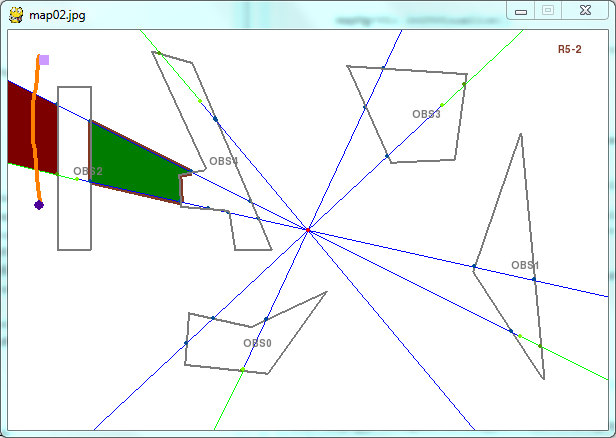
\includegraphics[width=\textwidth]{fig/regionlabel1.png}
		\caption{Labeling the regions}
		\label{fig:region_label:label}
	\end{subfigure}  
	%\\
	\begin{subfigure}[t]{0.47\linewidth}
		\centering
		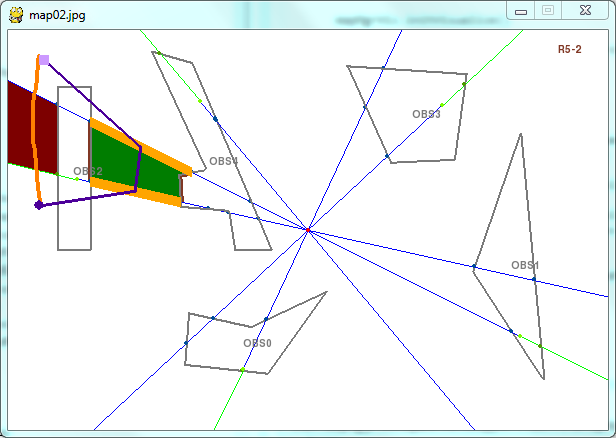
\includegraphics[width=\textwidth]{fig/regionlabelhomo1.png}
		\caption{Homotopy class satisfies the labeled regions}
		\label{fig:region_label:constraint}
	\end{subfigure}   
	\caption{Labeling region to generate homotopic constraints.}
	\label{fig:region_label}
\end{figure}

The nodes of the negative regions are forbidden to visit in the search on the topological graph.
A breath first search on the topological graph can return a set of string classes that satisfy the labeled constraints, which also implies a set of homotopy classes. 
%By the homotopic grammar, a set of string classes can be obtained from a set of homotopy classes.
The \textsc{HomotopyCheck}() in the exploration of the HA-RRT$^{*}$ will be defined by these string classes.
The problem is then similar with that in Section \ref{sec:string_constraint}.
Because only the optimal path in all these homotopy classes is wanted, a single-directional tree structure of the HA-RRT$^{*}$ is also enough to explore the working space.
The path returned by the HA-RRT$^{*}$ is the optimal solution under the labeled constraint.

\subsection{Homotopy classes with preference}
\label{sec:with_preference}

Sometimes there exists no hard constraint on the topology of the paths.
But there does exist the difference on different topology.
For example, visiting some region benefits some sub-task, or going around some object enhances the task performance.
If the human can tell the preference on the topology, scores can be assigned to each homotopy class.
In this case, the homotopy-based path planning returns a set of optimal paths in the homotopy classes.
Thus, a bi-directional tree structure is needed in the HA-RRT$^{*}$.
The problem can be viewed as a two-objective optimization problem.
One is the objective to be optimized, the other is the human's preference.

\begin{figure}
	\centering
	\begin{subfigure}[t]{0.47\linewidth}
		\centering
		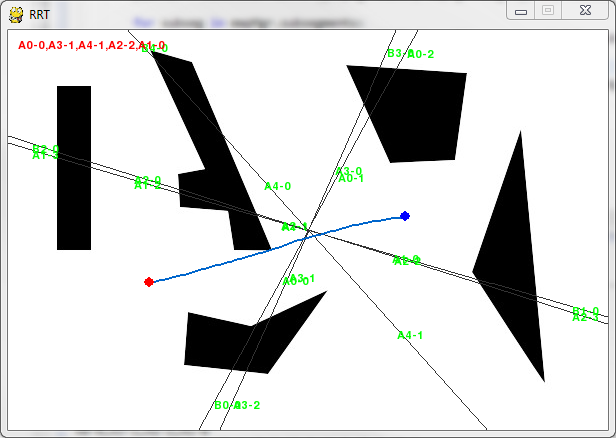
\includegraphics[width=\textwidth]{fig/screenshot1/all_homotopy1.png}
		\caption{Best path in one homotopy class.}
		\label{fig:all_homotopy:01}
	\end{subfigure}  
	%\\
	\begin{subfigure}[t]{0.47\linewidth}
		\centering
		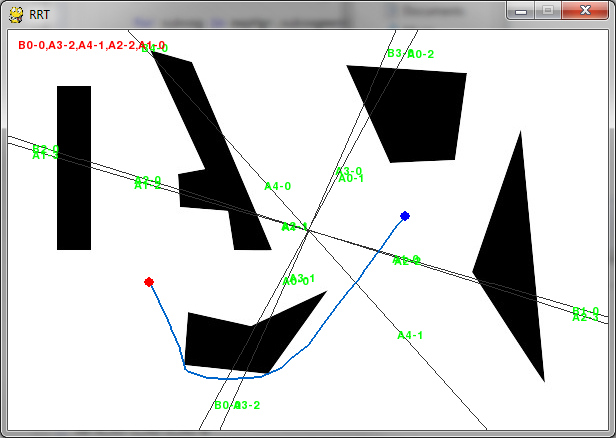
\includegraphics[width=\textwidth]{fig/screenshot1/all_homotopy2.png}
		\caption{Best path in one homotopy class.}
		\label{fig:all_homotopy:02}
	\end{subfigure}
	\\
	\begin{subfigure}[t]{0.47\linewidth}
		\centering
		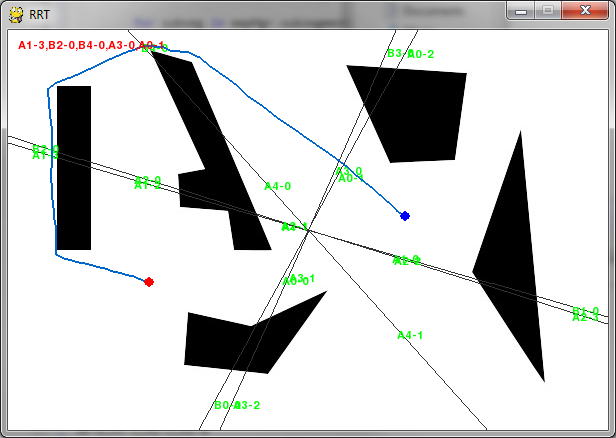
\includegraphics[width=\textwidth]{fig/screenshot1/all_homotopy3.png}
		\caption{Best path in one homotopy class.}
		\label{fig:all_homotopy:03}
	\end{subfigure}  
	%\\
	\begin{subfigure}[t]{0.47\linewidth}
		\centering
		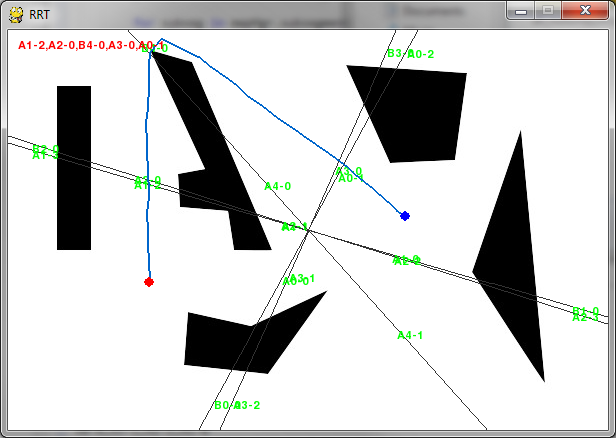
\includegraphics[width=\textwidth]{fig/screenshot1/all_homotopy4.png}
		\caption{Best path in one homotopy class.}
		\label{fig:all_homotopy:all_scores}
	\end{subfigure}	   
	\caption{Bidirectional RRT$^{*}$.}
	\label{fig:all_homotopy:no_pref}
\end{figure}

Figure \ref{fig:all_homotopy:no_pref} provides an example of the optimal paths in four homotopy classes.
Because the optimal solution in one homotopy class dominates all other solutions in the same class.
By combining the optimal paths in all the homotopy classes, we can find the non-dominated paths from them.
Figure \ref{fig:homotopy_human_interaction:pareto_score} illustrates such a Pareto front.

\subsection{Homotopy classes without preference}
\label{sec:without_preference}

Sometimes inherently the user has a mind of the topology preference but is too fuzzy to describe.
If the topology is included to have a two-objective optimization problem, it means that the optimal paths in all the homotopy classes are non-dominant.
Thus the HA-RRT$^{*}$ returns the optimal paths of all the homotopy classes.
Figure \ref{fig:homotopy_human_interaction:all_scores} gives an example of the scores.
With the interface of visualizing the optimal path in different homotopy class, the human can select one from them that matches his intent most.

\begin{figure}
	\centering
	\begin{subfigure}[t]{0.47\linewidth}
		\centering
		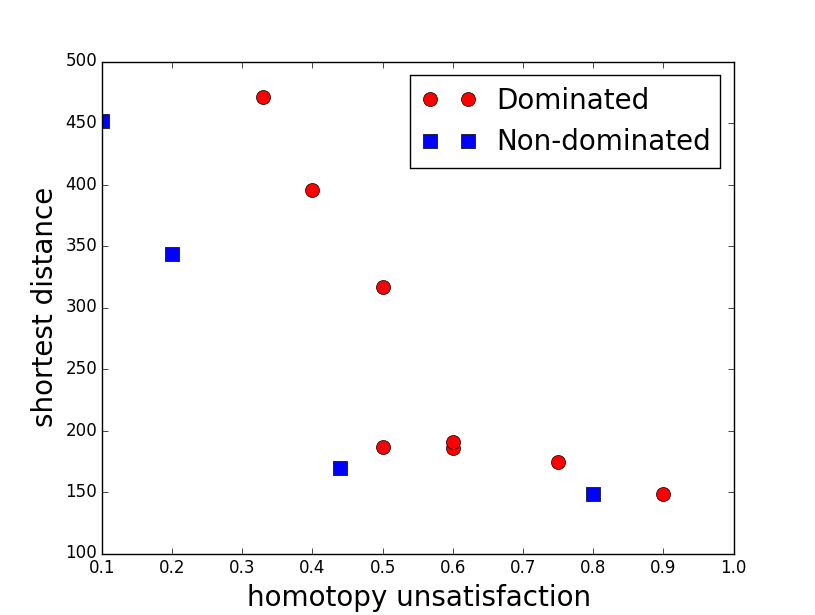
\includegraphics[width=\textwidth]{fig/pareto_score.png}
		\caption{Pareto front with topology preference.}
		\label{fig:homotopy_human_interaction:pareto_score}
	\end{subfigure}  
	%\\
	\begin{subfigure}[t]{0.47\linewidth}
		\centering
		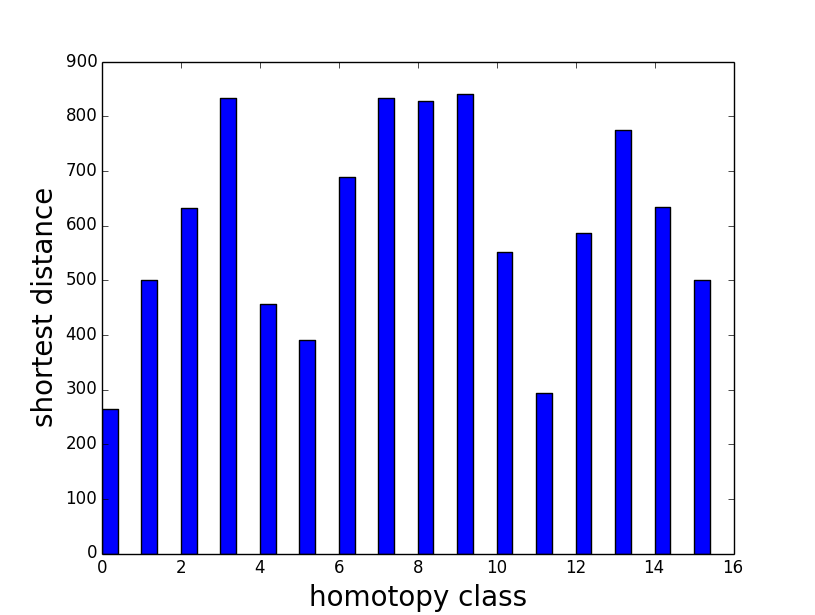
\includegraphics[width=\textwidth]{fig/all_homotopy_score.png}
		\caption{Minimum cost in all the homotopy classes.}
		\label{fig:homotopy_human_interaction:all_scores}
	\end{subfigure}   
	\caption{Interactive optimization.}
	\label{fig:homotopy_human_interaction}
\end{figure}


\section{Conclusion}
\label{sec:conclusion}

In the homotopy-based path planning, the homotopy classes can either be used as the constraint or the category of optimal search.
The HA-RRT$^{*}$ wares the string class of each branch in the exploration process, which indirectly attains the homotopy awareness with the assistance of the homotopic grammar.
The homotopic grammar can be used to determine the string classes in the same homotopy class.
With the string classess to represent the homotopy class, we can check whether a path satisfies a homotopic constraint 
or identify the homotopy class that a path belongs to.

The homotopic grammar can support the determination of the homotopy class 
However, the limitation of the RRT$^{*}$ leads to that the HA-RRT$^{*}$ cannot well support when the optimal path is not a simple path, which means that the path has at least one self-intersection.
In most of minimization problems, the optimal solutions are only in the simple homotopy classes.
If some scenarios need more than simple homotopy classes, 
the problem can be solved using the non-orientable surface like in \cite{Hershberger199463}.

When only single optimal solution is to be found, a single-directional RRT$^{*}$ can be enough to find the optimal path.
However, a bidirectional tree structure can accelerate the convergence rate, like in \cite{starek2014bidirectional}.
When the optimal solutions of more than one homotopy class is to be found, the bidirectional RRT$^{*}$ is required so that each position can have the optimal-to-come sub-path and optimal-to-go sub-path.
By using a bidirectional structure, the asymptotic optimality in each homotopy class can also be guaranteed.

The HA-RRT$^{*}$ enables the sliding autonomy to support different level of task supervisor's intent on the topology in planning paths.
The way of communication is also more natural to the human, because the human can directly visualize the path ``shape'' instead of converting to the quantitative format that a robot understands.
It also supports the application of more complicated tasks, especially when there is requirement on the topology of the paths in a complex map.
The homotopy-aware RRT$^{*}$ can be introduced to the multi-objective optimization to cover the increasing complexity of the tasks to the robots.
Also an online identification of the human's intent might start the workspace reduction earlier so that the efficiency could be enhanced.

\bibliographystyle{IEEEtranS}
\bibliography{reference}

\end{document}